\chapter{Results and performance}

\begin{figure}[H]
    \begin{center}
    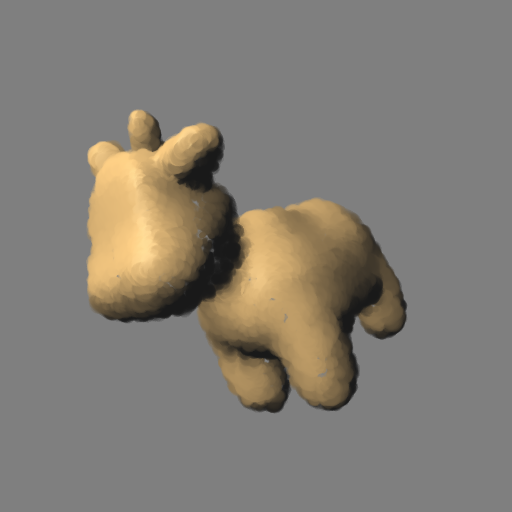
\includegraphics[width=70mm, height=70mm]{Resultats/spotPoint/final.png}
    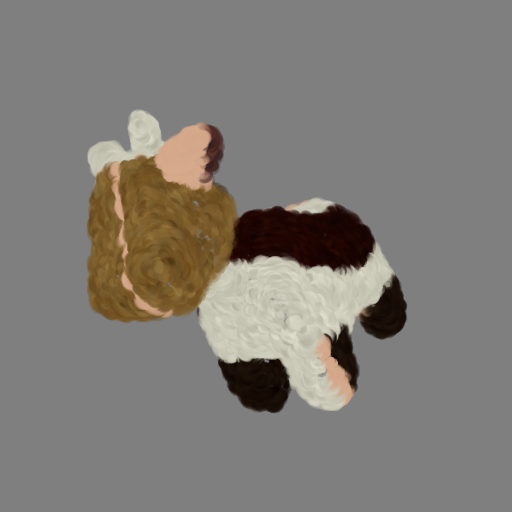
\includegraphics[width=70mm, height=70mm]{Resultats/spotPoint/final2.png}
    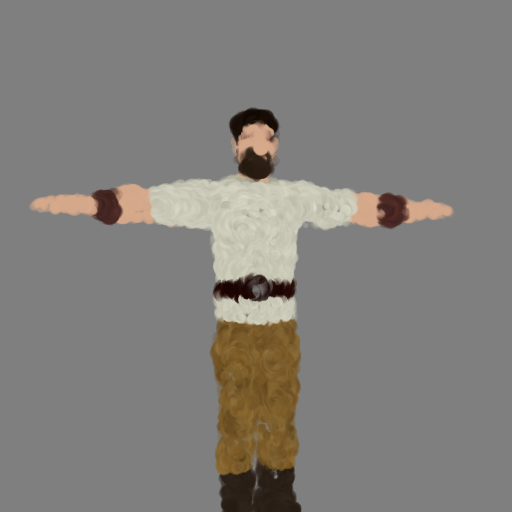
\includegraphics[width=70mm, height=70mm]{Resultats/pointCharacter/final.png}
    \end{center}
    \caption{Results of pointillism.}
    \label{results_point}
\end{figure}

\begin{figure}[H]
    \begin{center}
    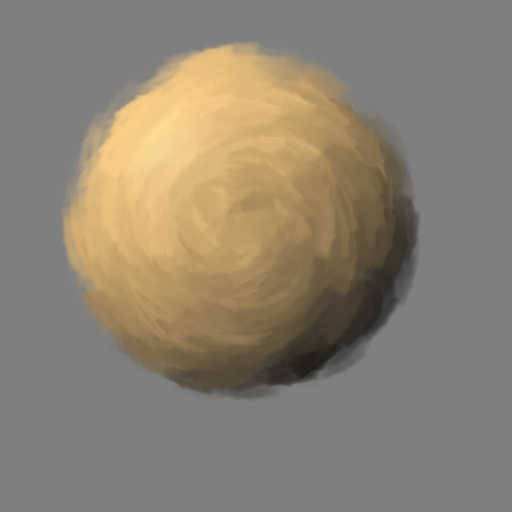
\includegraphics[width=70mm, height=70mm]{Resultats/painting1/final.png}
    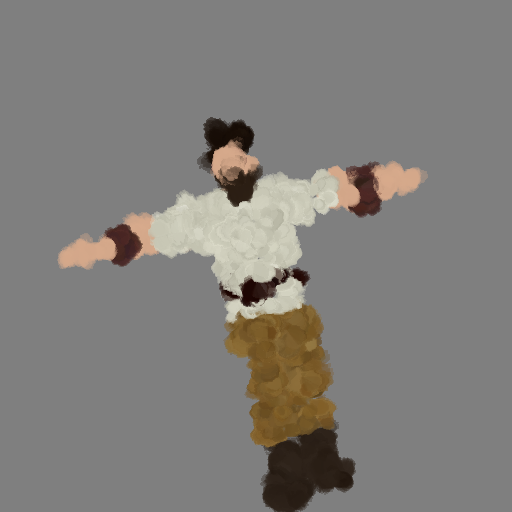
\includegraphics[width=70mm, height=70mm]{Resultats/paintChar/final.png}
    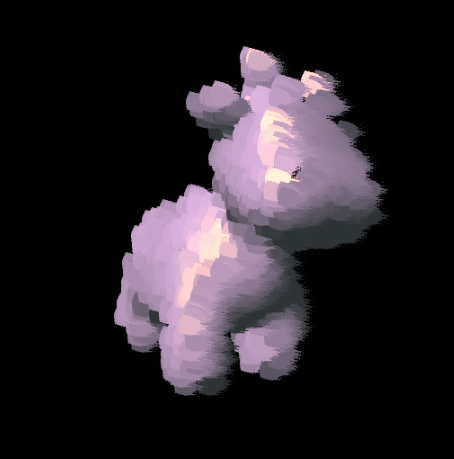
\includegraphics[width=70mm, height=70mm]{Resultats/spotPaint.png}
    \end{center}
    \caption{Results of brush painting.}
    \label{results_paint}
\end{figure}

\begin{figure}[H]
    \begin{center}
    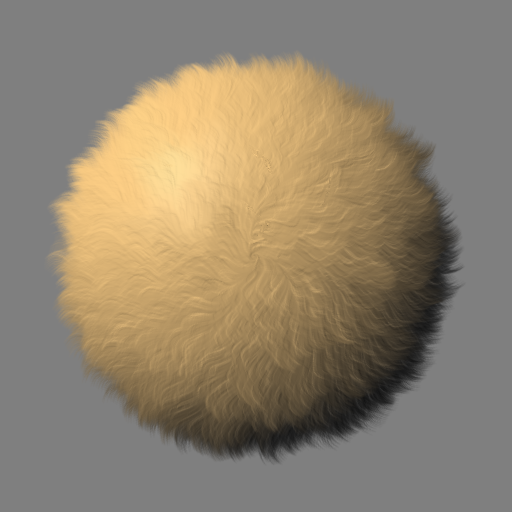
\includegraphics[width=70mm, height=70mm]{Resultats/bouledepoil1/final.png}
    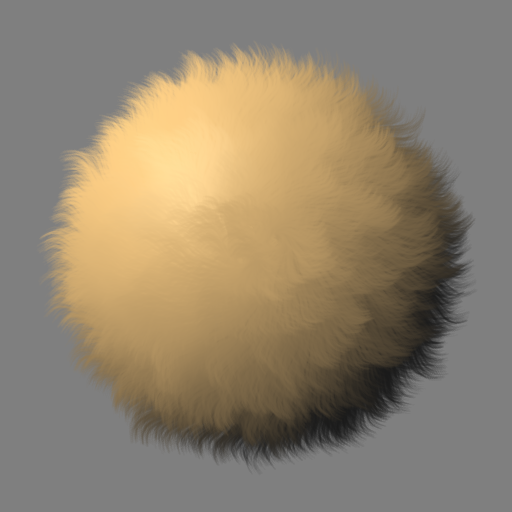
\includegraphics[width=70mm, height=70mm]{Resultats/bouledepoil2/final.png}
    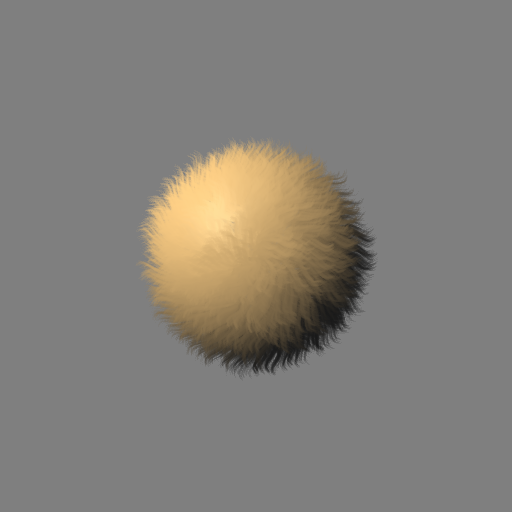
\includegraphics[width=70mm, height=70mm]{Resultats/bouledepoilFractalized/final.png}
    \end{center}
    \caption{Results of hairs rendering.}
    \label{results_hairs}
\end{figure}


Here there are some results of our method of stylization. The figure \ref{results_point} show some rendering with a point as mark and with different colors and models. We use the dot splat (the first in the figure \ref{splat_examples}) with a small size in order to keep a good level of details. In the figure \ref{results_paint} we tried to stylize as painted with brushes so we used brush stroke as splat. In the figure \ref{results_hairs}, we tried to render hairs with our technique we a simple hair as splat. We rotated it according to the normals and to increase the realism we changed the size of the splat depending on a procedural noise to have in some areas of the object smaller splat and in some others areas bigger splat. In our work, we did not focus on the color of rendered color because it depends on the 3d model and because our solution tends to be integrated into more complex pipeline rendering where the color is computed before.\newline

\textbf{Animations}

During our analysis of the state of the art, we talked about what happened if the camera moves. We made some videos to show the results of our solution with an animated camera. The videos are in the Maxime's website (\href{http://www.maximeisnel.fr/procedural-stylization/}{http://www.maximeisnel.fr/procedural-stylization/}). It is difficult to create a good \textit{flatness} effect while moving, the animations of the brush painting is a good example at each frame we have something that has good \textit{flatness} but during the motion we can see problem of \textit{temporal continuity}. This due to the alpha blending and also mainly due to the size of the splat because they are big and so to improve \textit{temporal continuity} we have to make to splat disappear/appear more slowly in order resolve some popping effect of the splats. As you can see in the animations of hairs rendering the splats are smaller so we don't have this problem of \textit{temporal continuity}. \newline


\textbf{Performance}

Our pipeline is implemented as a set of (non-optimized) OpenGL fragment shader in the Gratin software (\cite{vergne:hal-01254546}). Its performance is affected by the number of sampling during the creation of the procedural noises to minimize aliasing problem (popping effects). But the pipeline is mainly affected by the splatting step and the algorithm of order-independent transparency because in order to stylize the whole object we draw a lot of splat on the image so we have many splat cover others and then in order to know the order of them depending on the depth we sort with a \textit{bubble sort} an array that contains at most 300 elements (arbitrary limits fixed depending on the GPU used) for each pixel of the final image. In other words, the performance depends on how many splats are drawn and their size, if the size of splat is big the splats will cover more splats that if their size is small and the complexity will be higher. For the animation of brush painting (present in Maxime's website) with 300 frames with a resolution of 512x512 pixels, it takes approximately 4 minutes with an Nvidia GeForce RTX 2070 graphics card to render.






%%%% results
% several example with differents splats
% use noise to change the size of the splats in the object
% use tangents/normals map to rotate the splats
% differents shading



%%%% PERF
% nom de la carte
% resolution de l'image
% non-optimized
